\documentclass{standalone}
\usepackage{tikz}
\begin{document}
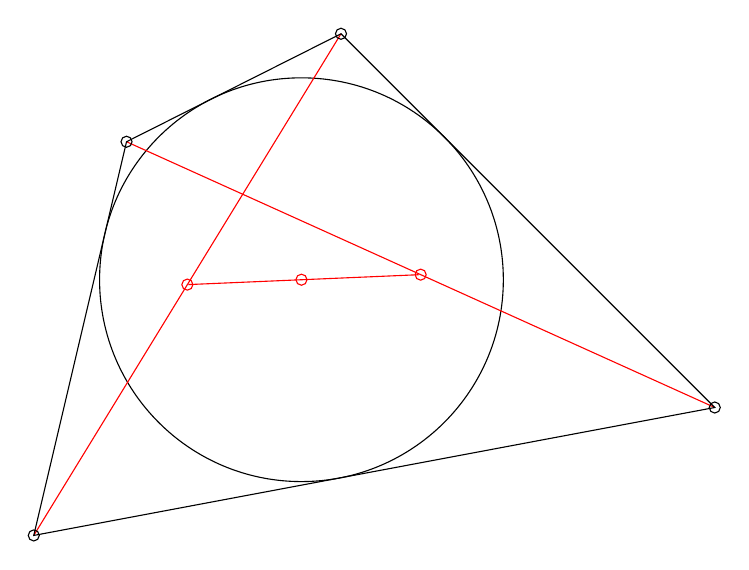
\begin{tikzpicture}[x=1pt,y=1pt]
\draw (120.06,-105.95) circle (72.95);
\draw[red] (79.22,-107.71) -- (162.41,-104.15);
\draw[red] (56.85,-56.10) -- (269.41,-152.13);
\draw[red] (23.33,-198.36) -- (134.35,-17.08);
\draw[red] (120.06,-105.95) circle (2.00);
\draw[red] (163.13,-104.12) circle (2.00);
\draw[red] (78.83,-107.72) circle (2.00);
\draw (134.35,-17.08) -- (56.85,-56.10) -- (23.33,-198.36) -- (269.41,-152.13) -- cycle;
\draw (134.35,-17.08) circle (2.00);
\draw (269.41,-152.13) circle (2.00);
\draw (23.33,-198.36) circle (2.00);
\draw (56.85,-56.10) circle (2.00);
\end{tikzpicture}
\end{document}
